\documentclass{school-22.211-notes}
\date{May 9, 2012}

\begin{document}
\maketitle

\lecture{Reconstruction/De-homogenization Methods} \label{de-homogenization}
In this lecture we consider given a homogenized solution, how to we re-construct the heterogeneous solution. Three references: Scott Palmtag's MIT PhD thesis `Advanced Nodal Methods for MOX Fuel Analysis' for good detailed math, Ken Rempse' NSE paper `SIMULATE-3 Pin Power Reconstruction: Methology and Benchmarking,' Qunlei Jiang's NCS MS thesis for detailed plots of complex terms `Intra-nodal Study for the Mixed LEU-MOX Cores.' 



\topic{Superposition Assumptions}
Basically we assume that the detailed flux distribution can be approximated by superposition of homogeneous nodal fluxes and lattice fluxes. That is, 
\eqn{ \phi_g^{het} (x,y) &= \phi_g^{hom}(x,y) \phi_g^{SA} (x,y) }
Keep in mind that, as the example in Fig.~\ref{dehom-supercomposing}, the heterogeneous flux should be continuous acorss the material boundary now, 
\eqn{\left. \phi_g^{SA, UO2} (x)  \phi_g^{hom, UO2} (x) \right|_{x=0} = \left. \phi_g^{SA, MOX} (x)  \phi_g^{hom, MOX} (x) \right|_{x=0} }
\begin{figure}[ht]
  \centering
  \includegraphics[width=4in]{images/methd/dehom-supercomposing.png}
  \caption{Supercomposing Thermal Flux in a 1D UO2/MOX problem} \label{dehom-supercomposing}
\end{figure}
Extensions:
\begin{itemize}
\item The above equation is for 1D. We reconstruct in 2D and 3D. 
\item The above equation is for flux, we reconstruct pin power too, in which case we need to know the pin-wise fission cross section form functions as well as the group-wise flux form functions. This would be a lot of data considering that form function, like cross sections and discontinuity factors have to be built into giant libraries vs. burnup, temperature, density etc). 
\end{itemize}

Consequently, most often powers are reconstructed be approximated by a superposition of homogeneous nodal powers and lattice pin powers. 
\eqn{ P^{het} (x,y) = P^{hom} (x,y) P^{SA} (x,y) }
where
\eqn{ P^{hom} (x,y) = \Sigma_{f1}^{hom} (x,y) \phi_1^{hom} (x,y) + \Sigma_{f2}^{hom} (x,y) \phi_2^{hom} (x,y) }
For detailed pin power reconstruction, one needs 2D $(x,y)$ shapes of fluxes -- which are not directly available. Nodal methods only provide flux shape information for the 1D shape in each direction. Cross section shapes are also only 1D averages. 


FIXME: If we want to do pin power reconstruction in our current frame-work, we need to store four form functions, two for flux and two for cross sections. Also be careful about fission rates, power and heat conducted. 


\clearpage
\topic{Non-Separable Flux Expansion}
FIXME: $f_m, f_n$ are just polynomials. 4th order polynomial has 25 terms. The point is, we do not need the exact shape in thermal group, so we can choose not to reconstruct until we need to. 
\begin{enumerate}
\item We asume nodal solution is known and construct a non-separable flux expansion for each group, analogous to the 1D SANM expansions as the following:
\begin{figure}[ht]
  \centering
  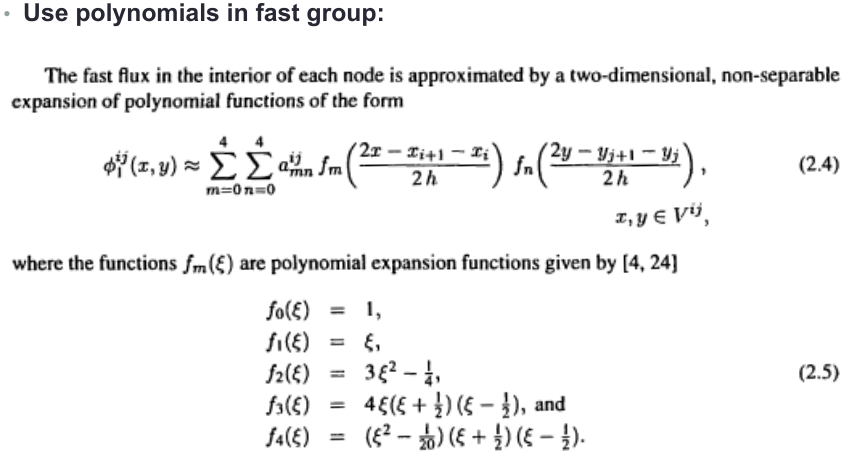
\includegraphics[width=5in]{images/methd/dehom-fast.png} 
  \\
  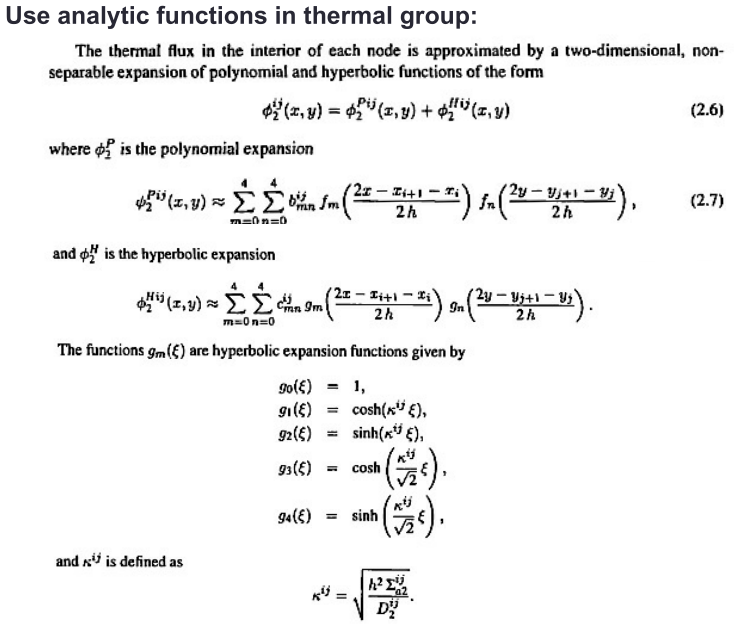
\includegraphics[width=5in]{images/methd/dehom-thermal.png}   
  \caption{Non-Separable Flux Expansion} \label{dehom-energy-group}
\end{figure}

\item Using 5th order polynomial, there are 25 unknown coefficients in the fast group ($a_{mn}$, where $m,n$ each goes from $0$ to $4$). For the thermal group, because of the polonomial and the hyperbolic functions, there appear to be 50 unknowns $b_{mn}, c_{mn}$; but it is really 25, because the other 25 for the specific colution can be solved from the fast group.

\item We have 9 constrains provided by the nodal solution, 
  \begin{itemize}
    \item 1 node average flux per group; 
    \item 4 surface-averaged fluxes per group;
    \item 4 surface-averaged net currents per group. 
  \end{itemize}
  
\item To supplement, the four corner point flux conditions are often used using the KWU method (non-iterative, second-order accurate): 
  \begin{itemize}
    \item Assume fluxes have quadratic shape on each node surface;
    \item Constrain average surface value to be the known nodal surface-averaged flux;
    \item Demand continuity of current in x-direction at the corner point; 
    \item Demand continuity of current in y-direction at the corner point;
    \item Perform post-nodal iteration to simultaneously determine all corner point fluxes;
  \end{itemize}

\item For each energy group, we have $9 + 4 = 13$ constrains and 25 unknowns. What we do is that we disregard the 12 highest order cross terms. 
\end{enumerate}

\clearpage
\topic{Corner Point Constraints}
Nodal corner-point fluxes are approximated by assuming that intra-nodal flux distributions are separable: 
\eqn{ \phi_{g,i,j}(x,y) = \frac{\phi_{g,i,j} (x) \phi_{g,i,j} (y)}{\bar{\phi}_{g,i,j}} }
Since the expansion has been performed about the corner point, the error in each estimator of the corner-point flux can be determined to be second-order; for instance, one of the corners has an error like, 
\eqn{ \epsilon = \frac{1}{4 \phi_{cp}} \frac{\partial \phi}{\partial x} \frac{\partial \phi}{\py} - \frac{1}{4} \frac{\partial^2 \phi}{\px \py} + O \left( \frac{\partial^3 \phi}{\partial^3 u} \right) }
Another important point is that the \textit{heterogeneous corner point flux has to be continuous}. Thus we need corner point ratios that are analogous to discontinuity factors that can be edited from lattice calculations. The corner point form function $\phi_{g,i,form, fet}^{cp}$ is coming from the lattice code. 


\begin{itemize}
\item In the general case, the corner-point fluxes are determined by averaging the four estimates of the heterogeneous corner-point flux, $cp$ is corner point, 
  \eqn{ \phi_g^{het,cp} &= \frac{1}{4} \left[ \phi_{g,i,j}^{hom,cp} \phi_{g,i,j}^{fct,cp} + \phi_{g,i+1,j}^{hom,cp} \phi_{g,i+1,j}^{fct,cp} + \phi_{g,i,j+1}^{hom,cp} \phi_{g,i,j+1}^{fct,cp} + \phi_{g,i+1,j+1}^{hom,cp} \phi_{g,i+1,j+1}^{fct,cp} \right] }

\item In order to satisfy the continuity conditions of reconstructed fluxes, the best-estimate homogeneous corner-point fluxes for each node are computed by, 
  \eqn{ \hat{\phi}_{g,i,j}^{hom,cp} = \frac{\phi_g^{het,cp}}{\phi_{g,i,j}^{fct,cp}} }
  The reconstructed corner point fluxes are then continuous. \textbf{CP ratio is the corner point analogue of ADF for assembly edges.}
\end{itemize}
Surface constrains preserve flux shape. Each corner has 4 surfaces connected to it. 


FIXME: this reconstruction method works for PWRs because the heterogeneous terms cancel out, whereas this is not the case for BWRs. This leads to Studsvik's separable corner point estimator: 


\clearpage
\topic{Basic Reconstruction Steps}
\begin{enumerate}
\item Solve normal nodal model global equations.
\item Determine corner point fluxes: first obtain the corner point fluxes from nodal method, then re-compute them to satisfy continuity. 
\item Compute 2D fluxe expansions coefficients. 
\item Compute 2D fission cross section shapes.
\item Integrate flux shape times cross section shape over each pin cell location to get `homogenized' pin powers. 
\item Evaluate lattice `pin power form function' at the nodal exposure. 
\item Multiply homogenized pin power by the pin power form function to get the `heterogeneous' pin powers.
\item Integrate the heterogeneous pin powers over time (usually exposure) to get heterogeneous pin burnups. Recent years there are trends to do this heterogeneous power separately in fast and thermal groups (in whatever number of groups that we need). 

\item Determine pin-wise thermal margins (DNBR, CPR, LHGR, etc). 
\end{enumerate}
For every axial node, we perform this reconstruction, and use an axial shape for getting the 3D distribution. The benefit of doing this two-step process (first solve things homogeneously, then re-construct) helps with water holes etc., because in the first 

gamma smearing affects Gd pins significantly. 



\clearpage
\topic{Homogeneous Cross Section Shape}




The reconstructed pin powers have errors. There are two spectral effect on cross sections we can correct for:
\begin{enumerate}
\item The first thing we want to check is the 2 group cross sections, which turn out to be only approximately correct as in Fig.~\ref{dehom-2g-err}. Errors arise from spatially constant cross section approximation, not from inadequancies of the spatial flux representations. This problem would go away if we use 10-ish energy groups instead of just 2 in a lot of people's nodal methods. More background: Lattice calculation uses 10-ish groups, nodal methods use 2 groups typically (SIMULATE uses 10-ish groups). The problem is, a \ce{UO_2} node and a MOX node by themselves would give a flat flux, and once we put them together in nodal method, there will be a large gradient at the interface of \ce{UO_2} and MOX (thermal flux decreases significantly from \ce{UO_2} to MOX). 
\begin{figure}[ht]
  \centering
  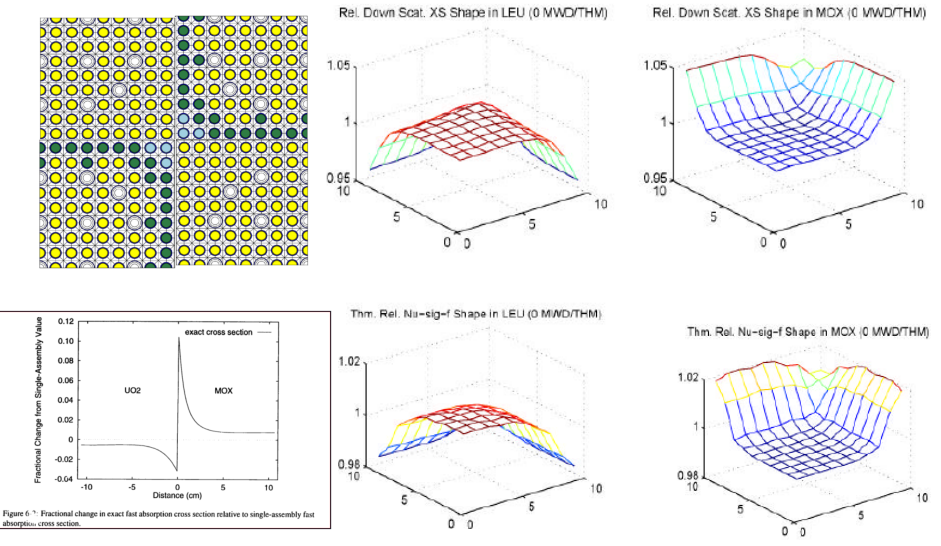
\includegraphics[width=5in]{images/methd/dehom-2gxs.png}
  \\
  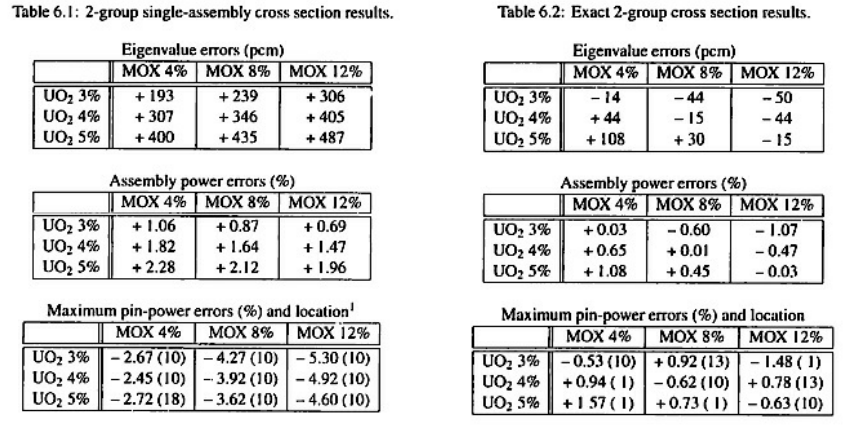
\includegraphics[width=5in]{images/methd/dehom-2gxs-err.png}
  \caption{2 Group Cross Section Errors} \label{dehom-2g-err}
\end{figure}
To adjust the cross sections, we use \hi{instantaneous leakage and spectral corrections}, where SA means single assembly, 
\eqn{ \frac{\Sigma_{\alpha 1}^B (x) - \Sigma_{\alpha 1}^{SA}}{\Sigma_{\alpha 1}^{SA}} &= B_{\alpha} \left[ \frac{-D_1 \nabla^2 \phi_1(x)}{\Sigma_{a1}(x) \phi_1(x) + \Sigma_{21} (x) \phi_1(x)} \right] } 
\eqn{\frac{\Sigma_{\alpha g}^S(x) - \Sigma_{\alpha g}^B(x)}{\Sigma_{\alpha g}^B(x)} &= \pm C_{\alpha g} \left| \frac{\Gamma(x) -\Gamma^{SA}}{\Gamma^{SA}} \right|^{P_{\alpha g}}  }
where $\Gamma(x) = \frac{\phi_2(x)}{\phi_1(x)}$. As in Fig.~\ref{approx-xs}, we can see the cross section after approximation corrections. 
\begin{figure}[ht]
  \centering
  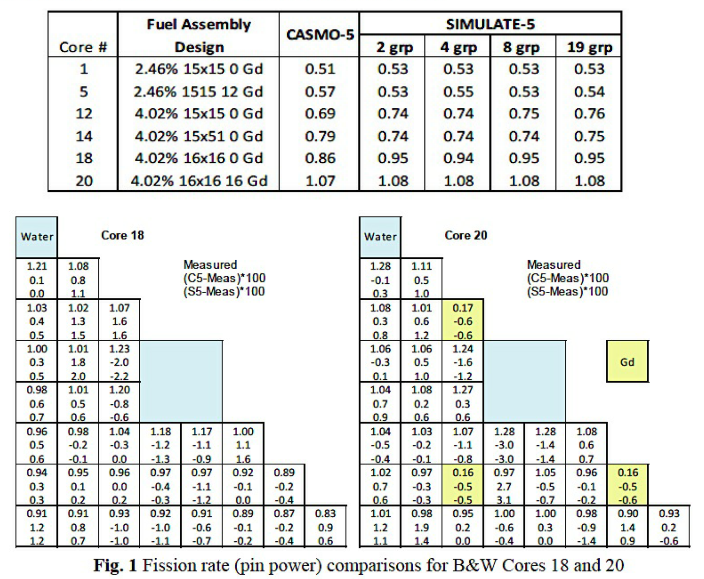
\includegraphics[width=5in]{images/methd/approx-xs.png}
  \caption{Approximate Cross Section Corrections vs. More Groups} \label{approx-xs}
\end{figure}
To measure power of a core, we pull out individual pins and measure the gamma deposited in it to get the power profile of it. The uncertainty comes out to be about 1.5\%, which is considered to be high precision. 

Advanced topic: fixing Cross-sections On The Fly/`Adhop' Method. 

This method is somewhat an empiracle one; hence it is not very robust. Nowadays, nodal methods just go to higher order of energy groups. 

\item Burnup effect on cross section: SH-1 etc. FIXME. 
\end{enumerate}

Sidenote: PWR tends to burn out the error because as the exposure increases, the faster spectrum 


\clearpage
\topic{SIMULATE-5 Radial Sub-Mesh Model}
We go from our lattice calculation to radial sub-mesh model, so we don't need to use xs and df from ....



\clearpage
\topic{Nodal Method Summary}
Basically a production-grade nodal code must have, 
\begin{itemize}
\item Accurate lattice data;
\item Coupling to an accurate thermal-hydraulic model;
\item Accurate nodal flux model;
\item Accurate re-homogenization model for cross section heterogeneity;
\item Accurate spatial cross section (homogenized) representation;
\item Accurate non-separable flux (homogenized) model;
\item Accurate pin power form functions;
\item Accumulated pin exposure models. 
\end{itemize}

\end{document}
